\documentclass[10pt]{article}
\usepackage[paperwidth=12cm,paperheight=6.4cm,margin=3mm]{geometry}
\usepackage{tikz}
\pagestyle{empty}
\pagecolor{white}

\begin{document}
\centering
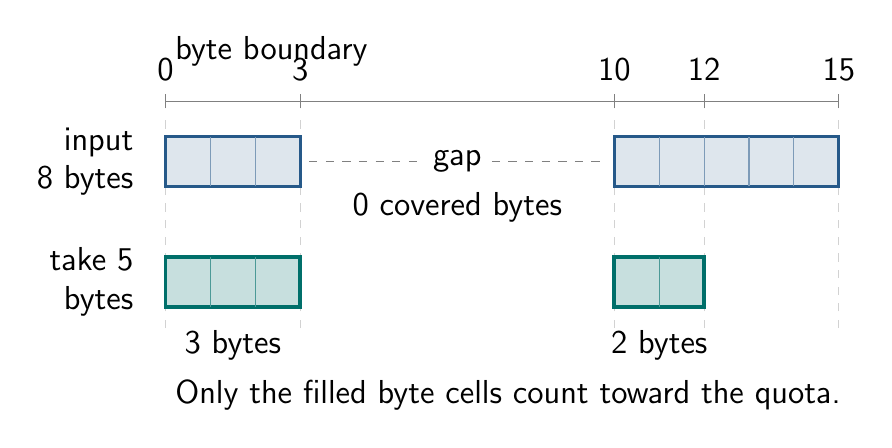
\begin{tikzpicture}[x=0.57cm,y=0.9cm,font=\sffamily\large]
  \definecolor{inputcolor}{RGB}{38,89,137}
  \definecolor{resultcolor}{RGB}{0,111,106}

  \node[anchor=west] at (0,4.8) {byte boundary};
  \draw[gray] (0,4.1) -- (15,4.1);
  \foreach \point in {0,3,10,12,15} {
    \draw[gray] (\point,4.0) -- (\point,4.2);
    \node[above] at (\point,4.25) {\point};
    \draw[gray!35,dashed] (\point,0.9) -- (\point,3.9);
  }

  \node[anchor=east,align=right] at (-0.5,3.25) {input\\8 bytes};
  \foreach \lower/\upper in {0/3,10/15} {
    \filldraw[fill=inputcolor!15,draw=inputcolor,line width=1pt]
      (\lower,2.9) rectangle (\upper,3.6);
  }
  \foreach \point in {1,2,11,12,13,14} {
    \draw[inputcolor!60] (\point,2.9) -- (\point,3.6);
  }
  \draw[gray,dashed] (3.2,3.25) -- (9.8,3.25);
  \node[fill=white,inner sep=3pt] at (6.5,3.25) {gap};
  \node at (6.5,2.6) {0 covered bytes};

  \node[anchor=east,align=right] at (-0.5,1.55) {take 5\\bytes};
  \foreach \lower/\upper in {0/3,10/12} {
    \filldraw[fill=resultcolor!22,draw=resultcolor,line width=1.4pt]
      (\lower,1.2) rectangle (\upper,1.9);
  }
  \foreach \point in {1,2,11} {
    \draw[resultcolor!70] (\point,1.2) -- (\point,1.9);
  }
  \node[below] at (1.5,1.0) {3 bytes};
  \node[below] at (11,1.0) {2 bytes};

  \node[anchor=west] at (0,-0.05) {Only the filled byte cells count toward the quota.};
\end{tikzpicture}
\end{document}
